%!TEX root = ../dissertation.tex
\begin{savequote}[75mm]
Simulation is a valid way of answering any question.
\qauthor{Professor Stephen Sekula}
\end{savequote}



\chapter{Introduction}
\label{introduction}

%***The past century has seen a great deal of progress and excitement in our understanding of nature through the success of the quantum revolution.
The advent of a quantum mechanical theory of nature revolutionized our physical interpretation of the surrounding world. Its success in resolving outstanding questions and making new predictions over the past century has cemented it as the cornerstone of our microscopic understanding of nature. However, even though the theory and mathematical framework developed is well understood, solving quantum mechanical problems on classical computers is often exponentially difficult\cite{Feynman1982}. Over the past few decades, a powerful set of experimental tools have been developed in a wide variety of atomic physics platforms that enable insight into testing fundamental properties of these theories. In fact, some platforms have sufficiently matured in development that private companies (e.g. Atom Computing\textsuperscript{\textregistered}, IonQ\textsuperscript{\textregistered}, Google\textsuperscript{\textregistered}, etc.) have begun their own research and development of these platforms to exploit their quantum mechanical properties for technological advancement. However, to appreciate the complexity of solving such quantum mechanical problems and their applicable virtues, we must first briefly discuss what properties we consider to be inherently quantum mechanical and their physical implications. 

\section{What we mean by ``quantum"}

%\footnotetext{\footnotemark a way to add footnotes to quotes}
\subsection{Single-body quantum}

Quantum mechanics was first realized as a necessary and accurate description of nature in the prediction of quantized energies of massless and massive single-bodied systems: e.g. energy of photons for black-body radiation\cite{Planck1914} and the prediction of the electronic energy levels of hydrogen\cite{Schrodinger1926}. This quantization resulted naturally for both systems due to the underlying constituents being described by a wave theory. Instead of these objects being described as point-like particles with properties whose values could change continuously, the boundaries of any given system admitted only a discrete set of solutions. This discreteness of these wave solutions meant the associated energies could also only take on discrete values with a bounded, non-zero lowest energy. 
%These results led to a successful description of the discrete possible orbitals an electron can occupy about an atom and has been shown to extreme precision by spectroscopic studies in atomic physics. 

This wave formulation, however, did more than just solve a few open problems in the early 20$^{\text{th}}$ century about the mismatch of nature's behavior with known classical theories. It further implied some fundamental distinctions between previous classical frameworks that have observable consequences. One such example comes from the Heisenberg uncertainty principle, which determines that, due to the wave nature of the physical constituent, there is an inherent uncertainty in the ability to define the constituent's physical properties: e.g. momentum and position -- any wave with a well defined momentum cannot have a well defined position and vice versa.\footnote{This is property is analogous to the Fourier transform: a delta function in any basis is maximally distributed among all degrees of freedom in its complementary, Fourier transformed basis. This comparison is relevant since it accurately describes the behavior of waves -- which all matter seems to be microscopically represented by.} This implies an inherent amount of fluctuations possessed by the quantum objects that are fundamental and can never be removed or ``frozen out". 

Another example results from the quantum mechanical discretization of the constituent's physical properties that render the possibility for multiple, independent objects to be fundamentally identical. In particular, if such identical objects are used as a resource for random variables, say coin flips, they will provide markedly different distributions from their classical counterparts.\footnote{The exact outcomes will depend upon the underlying quantum statistics of the objects themselves too: bosonic or fermionic, which depend on the symmetries of the quantum mechanical object and will not be described here.} Often however, our daily experience is among physics at high temperatures which provide a macroscopically large number of internal labels such that classical objects behave in accordance with the statistics associated with classical random variables, regardless of their underlying microscopic bosonic or fermionic nature.

%The lack of a continuous label for the properties of an object means that when two objects have the same labels they can never be distinguished from one another

\subsection{Many-body quantum}

However, perhaps the most famous consequence of quantum mechanics can arise from the interaction of multiple objects that then globally act as a wave.\footnote{This does not mean that many-particles act together simply like a single classical wave, like waves on the surface of water in the ocean. In this case all the particles are interacting with their neighbors through a linear response equation such that collective wave-like excitations can be made on the water. This classical wave is defined in a local, spatial basis where all interference in this wave happens only locally with itself or other waves. A many-bodied quantum wave function revolves around the global state itself having wave-like properties in the sense that it cannot be written as purely in a local basis and interference effects happen for this system on a global scale.} The implications of such behavior were recognized early on by Einstein, Podolsky, and Rosenstein in a Gedankenexperiment\cite{Einstein1935} of a pair of quantum mechanical objects whose internal properties are correlated. The correlations in this pair were famously shown by John Bell to generate physical implications for measured correlations that are indescribable by classical variables, which identifies these correlations as uniquely quantum \cite{Bell1964}. These quantum correlations between the two objects are qualitatively described by the term ``entanglement". 

This notion of entanglement leads to the concept of quantum many-body behavior that, as a whole, is described as a collective object with fundamentally wave-like properties. It additionally has a consequence that when measuring only some fraction of this many-bodied wave the remaining fraction's properties become described by a truly classical, statistical ensemble. The coherences related to the wave-like nature of the many-bodied function are erased and can produce truly classical outcomes. This development of classicality due to a lack of access to such global information provides a deep conceptual framework for understanding our macroscopic experience from our microscopic picture of nature. In particular, this has been useful for drawing a link between the agreement of thermodynamic properties from many-bodied classical systems in statistical mechanics and the behavior of a portion of a many-bodied wave function that behaves quantum mechanically \cite{Deutsch1991, Srednicki1994, Kaufman2016, DAlessio2016}. This suggests that it is not only the microscopic which behaves quantum mechanically, but the macroscopically large objects that we associate with classical laws of nature may actually naturally derive from the properties of many-bodied quantum mechanical systems -- we simply do not have access to the global system to verify it. 

%\begin{figure}[ht!]
%		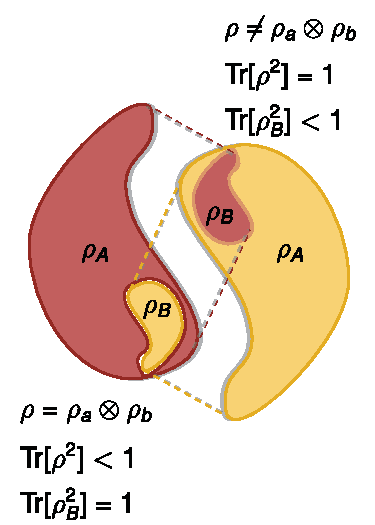
\includegraphics[width=\columnwidth]{figures/ch0/escher_fig_3.pdf} 
%		\caption{\textbf{Escher Fig. a,} }
%		\label{fig:BHP}	
%\end{figure}

%\begin{figure}
%\floatbox[{\capbeside\thisfloatsetup{capbesideposition={right,top},capbesidewidth=3 in}}]{figure}[\FBwidth]
%{\caption{\textbf{Classical correspondence to macroscopic quantum system. Red System,} This figure pictorially represents how classicality may derive from many-bodied, quantum mechanical behavior. The left object, $\rho$, represents our original classical system ($\text{Tr}[\rho^2]<1$) such as a thermal gas. Modern advancements of atomic physics allow experiments to locally cool a gas, $\rho_B$, down to its ground state such that it is both independent of the remaining gas, $\rho_A$, and can be described as a pure quantum state ($\text{Tr}[\rho_B^2]=1$). \textbf{Yellow System,} This locally quantum gas may be composed of many participating constituents. In general these, many-bodies may be highly-entangled such that if one measures, or only has access to a local part of the system, e.g. $\rho_B$, they will interact with a system that behaves like a classical distribution. In fact, generically, this system's local properties will even match those predicted by statistical ensembles constrained by thermodynamic quantities. The derivation of this local classicality do purely to the non-local quantum correlations of this many-body quantum system begs for the association/implication that perhaps we, along with the original gas, are simply classicality deriving from an astronomically large many-body quantum system.}
% \label{fig:escher}}
%{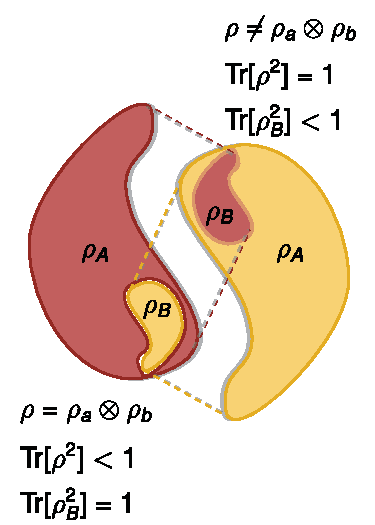
\includegraphics[width=2.5 in]{figures/ch0/escher_fig_3.pdf} }
%\end{figure}

\section{Quantum simulation: probing quantum many-body problems}

In many cases for large systems, physicists have found effective theories that allow for accurate descriptions of macroscopically large objects such that we may ignore the complexity related to its microscopic principles. This is often not the case for many-bodied quantum mechanical systems. Additionally, the overhead then necessary to analytically or numerically calculate results from the understood microscopic descriptions quickly makes these systems intractable. To circumvent this problem, a suggestion attributed to Richard Feynman \cite{Feynman1982} is to use a type of analog calculator for such systems, which would be known as a ``quantum simulator". The crux of the suggestion being that to successfully find the correct answers to quantum mechanical questions, one should use a system that is already inherently quantum mechanical such that it naturally simulates the correct answer.

Experimental atomic physics platforms have undergone significant technological maturity in the past few decades that make attempting such quantum simulations possible. Trapped atomic ion systems \cite{Blatt2012} and superconducting qubits \cite{Houck2012} enable high-fidelity control of few-particle systems with variable interaction strengths and geometries. These platforms harbor rapid experimental repetition rates that make them particularly promising for the purpose of quantum computation. However, they suffer from coupling to their surrounding environment: i) the static charge of atomic ions makes them sensitive to their surroundings due to the strength of the Coulomb force, and ii) superconducting qubits can be cooled down to extremely low temperature with dilution refrigerators, but are directly mounted to materials that harbor a finite phononic bath that can become relevant for the small energy gaps in many-body systems. This restricts their effective size in terms of quantum constituents and coherence times. New developments in waveguide manufacturing have enabled the study of correlated states in photonic systems and are well decoupled from their environment\cite{Garanovich2012}, but are not clearly scalable to the many-body limit. 

A powerful platform for probing such fundamental questions about many-bodied quantum mechanics is provided by ultracold atoms in optical lattices \cite{Bloch2008,Bloch2012}. The versatility of these platforms, thanks to the variety of available atomic species, enables exploring systems with both bosonic and fermionic statistics. These atoms can be cooled to their motional ground state and controlled microscopically with almost arbitrary potential energy landscapes on top of several optical lattice geometries while remaining isolated from their surrounding environment\cite{Lewenstein2012}. Their inter-atomic interaction strength can be tuned by orders of magnitude and even change signs via Feshbach resonances\cite{Chin2010}. Due to the convenient length scales in such systems, traditional microscopy techniques can be used to image both bosonic\cite{Bakr2009,Sherson2010,Miranda2015} and fermionic\cite{Haller2015,Parsons2015,Cheuk2015} species in optical lattices with single-site resolution, gaining access to local observables and correlation functions\cite{Endres2011} up to high orders\cite{Rispoli2018}.

% In the case of magnetic atoms (e.g. chromium, dysprosium, and erbium), an additional long-range dipolar interaction is accessible to p
%The versatility of optical lattice experiments with ultracold atoms have enabled studies of a canonical quantum many-body physics problem -- quantum phases and their transitions. 
One direction of quantum simulations with ultracold atoms concerns the realization of novel quantum phases of matter and the transitions between them. Pioneering studies have observed quantum phases of matter both in equilibrium \cite{Greiner2002,Jordens2008,Jo2009,Haller2010,Simon2011} and in driven, non-equilibrium\cite{Baumann2010,Landig2016,Choi2017,Leonard2017} systems. The majority of such experiments have focused on the quantum phases themselves and measure their order parameters through macroscopic observables. However, it is the transition of these phases in the critical regime that is exceedingly difficult to access owing to a divergence of correlations as quantum fluctuations reorder the system from phase to another \cite{Landau1937,Sachdev2011}. Only recently have ultracold atoms experiments probed such critical scaling behaviors for equilibrium quantum phase transitions near the transition point\cite{Anquez2016, Clark2016, Keesling2019}. 
%and is famously described by universal scaling behaviors within this traditional framework. 

\section{A non-equilibrium quantum phase}
 
A new class of non-equilibrium quantum phase transitions has recently emerged with behavior that is not captured by this conventional framework of equilibrium phase transitions. In the case of isolated quantum systems, these transitions occur among excited eigenstates in the system and can be understood by considering typical excited states individually  \cite{Nandkishore2015, Zvyagin2016, Tauber2017, Alet2018, Heyl2018}.\footnote{This is why these are sometimes referrred to as ``eigenstate phase transition" in the theory literature. } The experimental studies presented in this thesis will focus on two particular non-equilibrium quantum phases and their transition: \emph{quantum thermalization} and \emph{many-body localization}. These phases occur for isolated quantum systems that, while pure, are prepared far from equilibrium via a quantum quench\cite{Sakurai1993} and are identified by their inherent dynamics from coherently populating many excited eigenstates\cite{Nandkishore2015,DAlessio2016}. We exploit the microscopic access in our system to investigate one of the hallmarks of these quantum phases and their transition\cite{Amico2008,Bardarson2012, Nandkishore2015, DAlessio2016} -- entanglement properties of the many-body state. 

%requires knowledge of the structure of these individual eigenstates in the quantum system

A quantum thermalizing phase is predicted generically for interacting, non-integrable isolated quantum systems by the Eigenstate Thermalization Hypothesis\cite{Deutsch1991,Rigol2008,Jensen1985,Srednicki1994}. These systems harbor excited eigenstates which individually possess ergodicity among their local degrees of freedom and whose dynamics resemble those of a classical thermodynamic systems: agreement with statistical ensembles constrained only by global thermodynamic ensembles\cite{Jensen1985,Deutsch1991,Srednicki1994,Rigol2008} and maximization of local entropy. Often, such a system is difficult to simulate theoretically due to the generation of a large amount of entanglement during the ensuing dynamics \cite{Calabrese2005,Amico2008,Daley2012,Schachenmayer2013}. Atomic physics experiments, however, have been successful in observing such thermalizing behavior: the ergodic character of eigenstates has been observed in few-qubit systems\cite{Neill2016} and, as presented in this thesis, the role of entanglement\cite{Santos2012, Deutsch2013} in generating such locally thermal states\cite{Kaufman2016}.

The only known robust exception to this description is many-body localization (MBL)\cite{Nandkishore2015,DAlessio2016}. This exception can realized by the application of disorder to this thermalizing phase causes a breakdown of ergodicity and thermalization at a finite disorder strength by localization of this many-body, interacting system \cite{Anderson1958,Schwartz2007,Billy2008,Roati2008,Lahini2008,Deissler2010,Gadway2011,Kondov2011,Jendrzejewski2012,DErrico2008}. This breakdown can be understood as a fundamental change in the excited eigenstates, which results in  logarithmically slow entanglement dynamics throughout the system -- distinguishing these states as a separate non-equilibrium phase\cite{Pal2010,Huse2013}. Initial atomic experiments in this regime have tested the absence of thermalization by the memory of the initial states prepared far from equilibrium\cite{Schreiber2015,Smith2016,Choi2016}. This initial state localization is indeed a consequence of the many-body localized phase, but is not a unique characteristic\cite{Anderson1958,Nandkishore2015}. The results presented in this thesis provide evidence for such a unique characteristic by observing a logarithmically slow growth of correlations in the many-body state\cite{Lukin2019}. 

While both non-equilibrium phases are well understood theoretically and can be successfully described by phenomenological models\cite{Serbyn2013b,Huse2014,Nandkishore2015}, the transition between these two phases remains an open question\cite{Grover2014,Vosk2015,Potter2015,Khemani2017,Alet2018,Abanin2018,Zhang2018}. Several experiments have probed slow transport properties through local observables near this critical regime\cite{Luschen2017,Bordia2017}. While such anomalous transport has been predicted theoretically\cite{Agarwal2015,Setiawan2017,Zhang2018}, identifying anomalous transport as quantum critical dynamics is experimentally challenging, since similar behavior can also originate from stochastic effects: inhomogeneities in the initial state\cite{Luitz2016} or the coupling to a classical bath \cite{Nandkishore2014,Luschen2017b}. We overcome these challenges in our experiment with our protocol by evolving a pure, homogenous initial state under unitary dynamics where we additionally utilize post-selection to exclude coupling to the environment by atom loss\cite{Luschen2017b,Lukin2019}. In the experiments presented in this thesis, we observe system-size dependent thermalization, anomalous transport, and correlations that span the entire system and persist up to high orders near the critical point\cite{Rispoli2018}. We additionally observe behavior in support of a proposed microscopic mechanism that leads systems at intermediate disorder strengths critically towards thermalization via a sparse resonant network\cite{Potter2015,Khemani2017,Rispoli2018,Herviou2019}. 

%. We investigate the development of entanglement entropy that mimics thermodynamic entropy for an isolated quantum system which locally thermalizes under its own unitary dynamics\cite{Kaufman2016}. We then investigate the only known robust exception to this thermalizing behavior by studying the onset of many-body localization due to disorder. We observe the breakdown of thermalization in this phase and the logarithmically slow growth of entanglement throughout the system, which identifies the localized system to be an interacting one\cite{Lukin2019}. Lastly, we investigate the role of correlations in the critical dynamics that emerge at high-orders where the system transitions from thermalizing behavior to many-body localization\cite{Rispoli2018}.
%
%
%
%In the context of this thesis, we will focus on a particular class of quantum phase transitions that do not occur in equilibrium. Equilibrium quantum phase transitions necessitate being near the ground state.. We will investigate systems with generic excited state 

\section{Outline}

A quick summary of these studies are shown below as organized by their chapter:

\begin{itemize}
 \item \S \ref{sec:ch1} serves as an introduction to and derivation of band physics associated with both solid state physics and neutral atoms in optical lattices. Additionally, this is then written in terms of the Bose-Hubbard model as an effective description. This serves as the underlying framework for all experiments in the thesis. Although, it is rarely explicitly referenced.
 \item \S \ref{sec:qgm} provides a brief overview of the quantum gas microscope as the experimental apparatus. This chapter focuses on many of the details about how the lattice physics in \S \ref{sec:ch1} is physically realized as well as experimental protocols for calibrating the parameters of the Bose-Hubbard model.
 \item \S \ref{sec:ch3} introduces the concepts of entanglement and metrics used to quantify it. In this chapter, we then describe both conceptually and experimentally, how quantum phase transitions are realized in this system and measurements of entanglement in such phases. This will be discussed first for the superfluid-to-Mott-insulator transition and then for the paramagnetic-to-antiferromagnetic transition in the transverse Ising model.
 \item \S \ref{sec:ch4} summarizes the results and expands the techniques used in \S \ref{sec:ch3} to investigate and realize a highly entangled quantum mechanical system that locally mimics a classical system -- both in local observables and entropy. At the same time: by utilizing a many-body interference technique the system can be verified to be describable by a single quantum mechanical wave function. These experiments are supported by the Eigenstate Thermalization Hypothesis, which predicts many thermodynamic behaviors emerge from entropy of entanglement generated by partial observation of a pure quantum mechanical system.
 \item \S \ref{sec:ch5} describes the only known robust exception to the generic prediction of locally thermalizing quantum mechanical systems -- many-body localization. We study the breakdown of this thermalization in an interacting many-body system due to the application of a finite disorder strength, which realizes such many-body-localized states. We additionally quantify the separation of entanglement in the system that enable the first observation of the identifying property of this system: logarithmically slow growth of entanglement entropy throughout the system.
 \item \S \ref{sec:ch6} describes the properties of the transition from a quantum thermalizing system to a many-body-localized one. This transition is the focus of recent interest in the study of non-equilibrium phase transitions. In this regard, both the thermalizing and many-body-localized systems represent the quantum phases of highly excited eigenstates. We measure the growth of high-order correlations at the critical point when thermalization breaks down. Additionally, the observed structure of correlations in the system provides evidence for the suggested mechanism of a sparse resonant network that governs these critically thermalizing systems.
\item \S \ref{sec:conclusion} concludes with a summary and proposal for studying the possibility of other mechanisms governing this phase transition -- a so called ``avalanche" mechanism. We additionally study the concept of localization in Fock space and its dynamic properties. 
\end{itemize}


%The use of ultracold atoms in optical lattices has been particularly successful with celebrated results including experimental realizations of many-bodied quantum wave functions undergoing quantum phase transitions \cite{Greiner2002}. The root of the success of this platform arising from its versatility in atomic properties, isolation from external environment, and maturity in technical implementation. The experimental architecture used for all experiments in this thesis is known as a quantum gas microscope\cite{Gillen2009} -- which has the additional feature of providing microscopic resolution of the many-bodied wave function and its spatial correlation functions.

%The degree of control and resolution of this apparatus will enable the detailed studies of how many-bodied quantum mechanical systems become entangled through the growth of quantum correlations provided by strongly interacting models. This thesis will use such measurements to probe the properties of entanglement and the emergence of collective fluctuations across equilibrium and non-equilibrium quantum phase transition. While we will briefly investigate the former, the latter is the focus of this research and represents a novel application of the concepts of quantum phase transitions beyond the ground states of quantum systems. Where the characteristic behavior of the system is now embedded in the characteristic non-equilibrium dynamics of the many-body system.

